\section{Mobile antennas}
\label{sec:mobile_antennas}
Mobile phones require antennas to communicate. This section introduces the general properties and characteristics of mobile antennas, including all necessary parameters and techniques used in the research of this thesis. Latter part of this section focuses on different antenna types that are used in mobile devices.

\subsection{Antennas in general}
\label{sec:general_antennas}
An antenna is the single most important part of a radio system. The purpose of an antenna is to transmit and receive radio waves. Thus, it is designed to transform guided electromagnetic waves to free space waves, and vice versa (see Figure \ref{fig:antenna_principle}) \cite{holopainen_phd}. As an electrical signal travels from one point to another via transmission line, e.g.\ coaxial cable or waveguide, the carried energy is bounded to the line or very nearby. Comparably, antennas work the other way: they are encouraging signals to propagate as far away from the antenna as possible, i.e.\ to radiate \cite{stutzman}.

\begin{figure}[H]
    \centering
    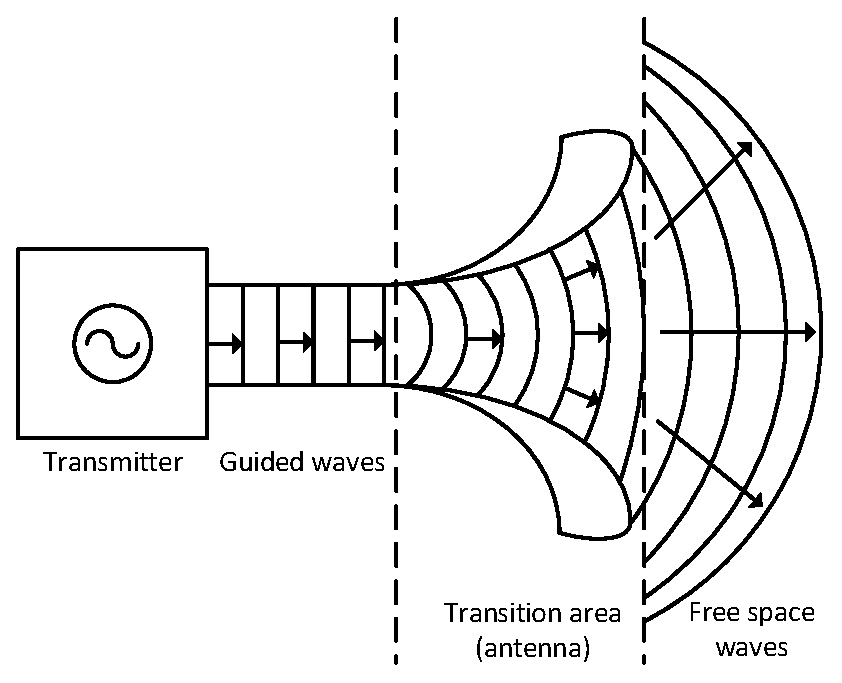
\includegraphics[width=0.7\textwidth]{img/antenna_principle.eps}
    \caption{Principle of antenna operating in transmission presented in \cite{saunders}.}
    \label{fig:antenna_principle}
\end{figure}

%how antennas radiate
Antennas radiate because of accelerated charges \cite{stutzman}. Acceleration causes disturbance that initiates electromagnetic fields to propagate away from the source of disturbance. The acceleration of charges occurs as change of speed or direction of the charge. As an example, a case of a single thin wire and single charge can be considered. Figure \ref{fig:charges} illustrates the following situations \cite{saunders, balanis}:
\begin{enumerate}
    \item Stationary charge will not create radiation, since there is no current (\ref{fig:no_move}).
    \item Charge moving with constant speed will not create radiation, if the wire is straight and infinitely long (\ref{fig:infinite}).
    \item Charge moving with constant speed creates radiation, if the wire is either curved (\ref{fig:curved}), bent (\ref{fig:bent}), discontinuous (\ref{fig:discont}), terminated (\ref{fig:terminated}), or truncated (\ref{fig:truncated}).
    \item Charge oscillating in a periodic motion creates radiation (\ref{fig:osc}).
\end{enumerate}

\begin{figure}[H]
    \centering
    \begin{subfigure}[b]{0.4\textwidth}
        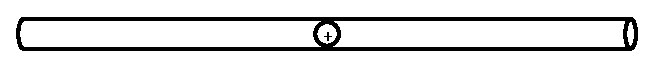
\includegraphics[width=\textwidth]{img/radiations_no_movement.eps}
        \caption{No radiation.}
        \label{fig:no_move}
    \end{subfigure}
    \begin{subfigure}[b]{0.4\textwidth}
        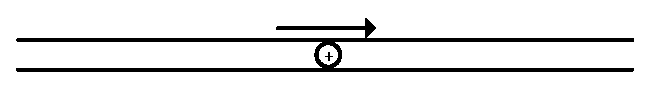
\includegraphics[width=\textwidth]{img/radiations_infinite.eps}
        \caption{No radiation.}
        \label{fig:infinite}
    \end{subfigure}
    
    \begin{subfigure}[b]{0.4\textwidth}
        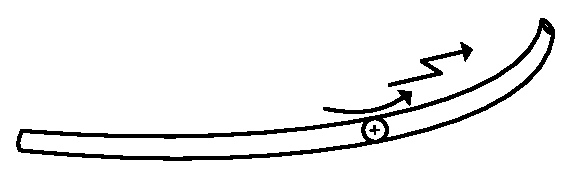
\includegraphics[width=\textwidth]{img/radiations_curved.eps}
        \caption{Radiates.}
        \label{fig:curved}
    \end{subfigure}
    \begin{subfigure}[b]{0.4\textwidth}
        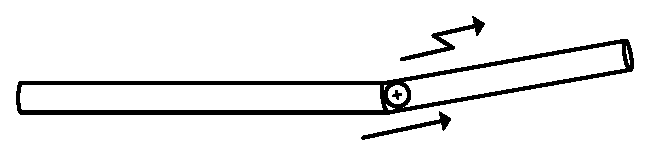
\includegraphics[width=\textwidth]{img/radiations_bent.eps}
        \caption{Radiates.}
        \label{fig:bent}
    \end{subfigure}
    
     \begin{subfigure}[b]{0.4\textwidth}
        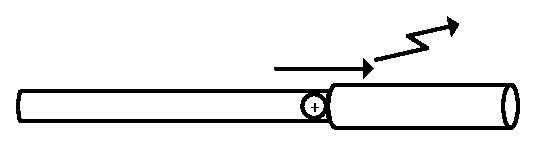
\includegraphics[width=\textwidth]{img/radiations_discont.eps}
        \caption{Radiates.}
        \label{fig:discont}
    \end{subfigure}
    \begin{subfigure}[b]{0.4\textwidth}
        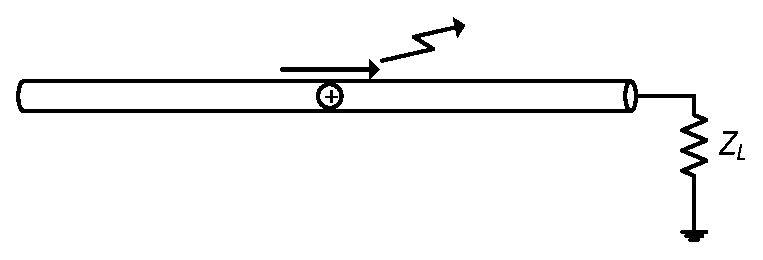
\includegraphics[width=\textwidth]{img/radiations_terminated.eps}
        \caption{Radiates.}
        \label{fig:terminated}
    \end{subfigure}
    
     \begin{subfigure}[b]{0.4\textwidth}
        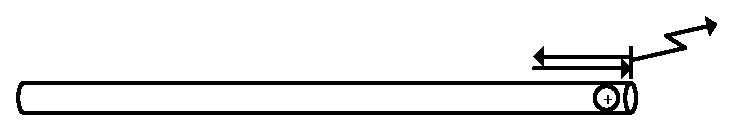
\includegraphics[width=\textwidth]{img/radiations_truncated.eps}
        \caption{Radiates.}
        \label{fig:truncated}
    \end{subfigure}
    \begin{subfigure}[b]{0.4\textwidth}
        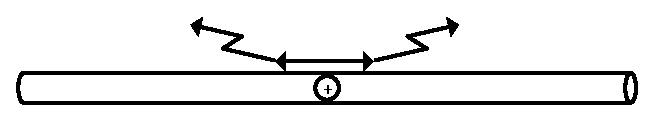
\includegraphics[width=\textwidth]{img/radiations_osc.eps}
        \caption{Radiates.}
        \label{fig:osc}
    \end{subfigure}
    \caption{Examples of charges producing radiation. Re-illustration from \cite{saunders, balanis}.}
    \label{fig:charges}
\end{figure}

These described situations are the most elementary examples of radiation. In real world, the normal case is a steady-state charge oscillating, usually sinusoidally, and the oscillation frequency equals to the radiation frequency \cite{stutzman}. Once accelerated charges have started a wave, they are not needed anymore. Wave can sustain itself by closing electric field lines on themselves, since there are no charges present. %\cite{stutzman}

Maxwell has discovered that fields surrounding a transmission line are guided by the line itself \cite{stutzman}. In open-ended transmission line, a standing wave is formed by the interaction between the incident wave and reflections. The standing wave has zero current at the end of the line and nulls every half wave length from there. The current flowing in transmission line wire are headed in opposite directions, which creates strong, constructive interference of electric and magnetic fields between the wires. Bending quarter-wave long parts from the ends of both wires outwards exposes the reinforced fields to open space. In the formed half-wavelength dipole antenna, the currents are flowing to the same direction and the maximum of its current distribution lies in between the halves \cite{stutzman}. Thus, antenna is a structure that radiates. %\cite{stutzman}

%when used
Radiated waves propagate away from the antenna, to all directions, although not uniformly as antennas do not have any guiding structures in contrast to transmission lines \cite{stutzman}. Antennas are preferred to transmission lines when either the operating frequency is high or distance between transmitter and receiver is large. Increment of either of those increases costs and signal losses of transmission lines, which often makes antennas and wireless transmission preferable choice. %\cite{stutzman}


\subsection{Requirements for mobile antennas}
\label{sec:small_antennas}
Mobile antennas are typical examples of small antennas. Small antennas can be defined a few different ways \cite{modern_small_antennas}. \emph{Electrically small antennas (ESA)} are not necessarily small in size, but they are small compared to wavelength. An ESA can be surrounded with a sphere of radius $r\leq\frac{\lambda_0}{2\pi}$, where $\lambda_0$ is the free space wavelength at operating frequency. An antenna can also be \emph{physically small (PSA)} if its measured dimensions are small. PSAs do not have any exact definition, rather than a sensual view of smallness. For this thesis, the main focus is on electrically small antennas.

As it was mentioned previously in Section \ref{sec:general_antennas}, antennas radiate on a certain frequency, called resonance frequency ($f_0$). The wavelength $\lambda_0$ is related to the frequency via propagation speed \cite{stutzman}, which in free space is the speed of light $c$
\begin{equation}
\label{eq:fcl}
    f_0 = \frac{c}{\lambda_0}.
\end{equation}
At resonance, a standing wave is formed at the antenna \cite{stutzman}. Since the resonance frequency is the same as the radiation frequency, the size of an antenna is related to the wavelength. For an electrically small antenna, the physical size of it is only a fraction of wavelength. Small electrical size results in small input resistance and large capacitive (or inductive for some antenna types) input reactance \cite{modern_small_antennas}. The input impedance of an antenna at resonance is (almost) purely resistive, and outside that frequency the impedance of an ESA is changing quickly and therefore being the main limiting factor for usable bandwidth \cite{holopainen_phd}. This characteristic makes wide band matching and achieving wide band performance difficult for electrically small antennas.

The three important characteristics of an electrically small mobile antenna are size, efficiency, and bandwidth, which are all interconnected \cite{holopainen_phd}. Wider bandwidth can be achieved with a larger antenna, which is not desirable in a modern mobile phone. Decreasing efficiency might increase bandwidth, but it would also decrease handset's battery life. Thus, improving one of these parameters is possible by worsening the others. The important challenge in small antenna design is to find a good trade-off between the three parameters for each application.

Antennas used in handsets and other handheld devices operate in demanding environment. Orientation of the phone is rather random, especially in standby mode. Signal between terminal and base station propagates in every way from line-of-sight to wide multipath arrival angles. Signal strength has to be adequate to counter fading from human head and hand. Hand-effect is a major problem for mobile antennas. Studies have shown that up to $70\,\%$ of the radiated power might get absorbed into user's hands \cite{valkonen_phd}. Generally, the requirements for mobile antennas can be listed in the following way \cite{saunders, lehtovuori_phd}:
\begin{enumerate}
    \item \textit{Radiation pattern:} Due to the randomly changing orientation of the phone, omnidirectional pattern in azimuth is desirable, as well as wide beamwidth vertically. Though, the precise pattern is not that important given the propagation environment and the proximity of the user.
    \item \textit{Input impedance:} Considering the number of used frequency bands today, phones have wide operational bandwidths. The antenna should be well matched to the source at all required bands.
    \item \textit{Efficiency:} Since omnidirectional antennas have low gain, it is critical to have good efficiency in order to transform input power to radiation. Efficiency might be the most important figure-of-merit for mobile antennas.
    \item \textit{Size:} Mobile devices consist of many subsystems, and nowadays require multiple antennas. Together with the constrained physical size of the handset, the antennas should be as small as possible. However, small size creates challenges as other requirements cannot be neglected.
    \item \textit{Manufacturability:} Mobile phone antenna is useless if it is not robust against mechanical damages or cannot be mass produced with reasonable costs. Also, antennas should fit the appearance requirements of the consumer product. 
\end{enumerate}

The following \Cref{sec:efficiency,sec:matching,sec:pattern,sec:bandwidth} discuss the first three of these requirements in more detail.

\subsection{Antenna impedance \& efficiency}
\label{sec:efficiency}
An antenna can be modeled with an electrical equivalent circuit consisting of two resistances and one reactance (Figure \ref{fig:antenna_equivalent}) \cite{stutzman,balanis,saunders}. One of the resistances represents ohmic and other losses ($R_o$) and the other is radiation resistance, $R_r$. It models the power loss from the circuit due to radiation, i.e.\ radiated power. Antenna's input impedance \cite{stutzman, balanis} is defined as
\begin{equation}
\label{eq:input_impedance}
    Z_a=R_a+\j X_a,
\end{equation}
where antenna resistance $R_a=R_o+R_r$ and $X_a$ is antenna reactance, which models the energy stored in the near-field of the antenna. %\cite{stutzman}

\begin{figure}[H]
    \centering
    \begin{circuitikz}[wave/.style={decorate,decoration={snake,post length=1.4mm,amplitude=2mm,segment length=2mm},thick}]
        \draw 
            (0,0) to[sI] (0,2)
            (0,2) to[R, l_=$R_s$] (2,2)
            (2,2) to[european resistor, l_=$X_s$] (4,2)
            (6,2) to[R, l^=$R_r$] (6,0)
            (0,0) to[short] (4,0);
        \draw [densely dashed] (4,2.7) to[short] (4,-0.7);
        \draw 
            (4,2) to[R, o-, l_=$R_o$] (6,2)
            (4,0) to[european resistor, o-, l^=$X_a$, n=res] (6,0)
            (5,-0.3) node[label={below:Antenna}]{}
            (2,-0.3) node[label={below:Transmitter}]{};
        \draw [->,wave] (6.7,1.7)--(7.7,2) node[]{};
        \draw [->,wave] (6.7,0.3)--(7.7,0) node[]{};
    \end{circuitikz}
    \caption{An equivalent circuit for a generator connected to an antenna. \cite{saunders}}
    \label{fig:antenna_equivalent}
\end{figure}

In the electrical equivalent circuit, the antenna is connected to a generator. Some of the input power $\sub{P}{in}$ is dissipated in ohmic losses, and only a portion of it, $\sub{P}{rad}$ is radiated. Radiation efficiency describes how much of the power is radiated, in other words utilized. The radiation efficiency \cite{pozar} is given as 
\begin{equation}
\label{eq:efficiency}
    \sub{\eta}{rad} = \frac{\sub{P}{rad}}{\sub{P}{in}} = \frac{R_r}{R_r+R_o}.
\end{equation}

Efficiency can also be approximated with system's $S$-parameters. As radiated power is considered as power lost from the system, all $S$-parameters of an $N$-port system are required when determining the radiated power. For a lossless system, efficiency for port $i$ \cite{lehtovuori_phd} can be expressed as
\begin{equation}
\label{eq:eff_aprx}
    \sub{\eta}{rad} = 1-\sum_{j=1}^{N}|S_{ij}|^2,
\end{equation}
where $S_{ij}$ are the scattering parameters expressing the power flow from port $j$ to port $i$. For other than lossless systems, this works only as an approximation due to e.g.\ substrate or ohmic losses \cite{lehtovuori_phd}.

Good efficiency may be the most important property for any antenna. An efficient antenna requires less power for transmitting a signal with desired field strength. Higher efficiency also improves antenna's Signal-to-Noise Ratio (SNR), which increases the signal quality in reception. Therefore, an efficient antenna can improve link quality and battery life of handset \cite{molisch}. In an ideal situation, $\sub{\eta}{rad}=1$. As mobile antennas operate on wide range of frequencies, this is impossible to realize, and the typical realized efficiency is in the range of $0.3$-$0.9$ \cite{volakis,ilvonen_phd}. %\cite{molisch}


\subsection{Radiation characteristics}
\label{sec:pattern}
Radiation pattern shows the far-field radiation properties of an antenna \cite{balanis, stutzman}. It tells the strength and phase of radiation in certain direction with respect to an isotropic radiator radiating the same energy \cite{balanis}. Isotropic radiator is physically unrealizable, but it is used as a reference of radiation characteristics due its definition: lossless antenna radiating equally to all directions \cite{balanis}. More realistic type is directional antenna \cite{balanis}, which radiates significantly more energy in some direction than in others. Special type of this pattern is referred to as omnidirectional \cite{balanis}, which has a nondirectional pattern in a given plane (usually azimuth plane) and directional in an orthogonal plane (usually elevation plane).

Usually the pattern is expressed as a function of the directional coordinates: azimuth angle $\phi$ and elevation angle $\theta$. Strengths of radiated electric or magnetic fields in the far-field are referred to field patterns, while the power density of them is power pattern. Often radiation patterns \cite{stutzman} are normalized to their maximum values
\begin{equation}
\label{eq:f_norm}
    F(\theta,\phi)=\frac{E_\theta}{E_\theta(\mathrm{max})},
\end{equation}
where $E_\theta$ is the $\theta$-component of the electrical field and $E_\theta(\mathrm{max})$ is its maximum value. For any radiating element, field patterns \cite{stutzman} can be expressed in a general form
\begin{equation}
\label{eq:f_gen}
    F(\theta,\phi) = g(\theta,\phi)f(\theta,\phi),
\end{equation}
where $g(\theta,\phi)$ and $f(\theta,\phi)$ are element and pattern factors, respectively. Pattern factor is an integral over the current distribution in space and element factor is the pattern of an infinitesimal current in the distribution \cite{stutzman}.

Generally, for a good communications link, it is useful to know how an antenna concentrates the radiated energy. Directivity describes this property. Normally, the word \textit{directivity} refers to the maximum directivity ($\sub{D}{max}$) of an antenna, but the parameter is actually dependent of the observation point. It is defined as the ratio of radiation intensity in a direction to the average intensity. Directivity \cite{stutzman} in a certain direction can be expressed with normalized power pattern 
\begin{equation}
\label{eq:dir}
    D(\theta, \phi) = \sub{D}{max}|F(\theta,\phi)|^2.
\end{equation}

Thus, directivity is purely directional characteristic determined by the power pattern of an antenna. As antennas are parts of a radio system, besides their ability to focus radiation to certain direction, also their capabilities of transforming power at input terminals to radiation is practical to know. The feature combining all this information is called antenna's gain. Since all of the input power is not radiated, and especially electrically small antennas are very inefficient, gain might be more useful than directivity in case of mobile antennas. Gain \cite{stutzman} is defined as 
\begin{equation}
    \label{eq:gain}
    G(\theta,\phi) = \sub{\eta}{rad}D(\theta,\phi).
\end{equation}

Mobile antennas typically have more or less omnidirectional pattern \cite{ying_mobile_antennas}, due to the fact, that a user cannot know where the nearest base station is. Since omnidirectional pattern is nondirectional in one plane, antennas of that type usually have low gain which makes efficiency even more important parameter for mobile antennas.

\subsection{Impedance matching}
\label{sec:matching}
As the primary objective of an antenna is to convert waves bounded to transmission line to free space waves, an antenna has to be matched to the source in order to avoid reflections. Matching also improves SNR of the system and reduces amplitude and phase errors \cite{pozar}. Reflections occur in the connection point of a transmission line and an antenna, and large reflections prevent maximizing radiated power in transmission or utilized power in receiving. Maximum power is obtained when an antenna is conjugate matched \cite{stutzman} to the source impedance $Z_s=R_s+\j X_s$ (or to load impedance, respectively)
\begin{align}
\label{eq:matching1}
    Z_s^* &= Z_a,\\
\label{eq:matching2}
    R_s-\j X_s &= R_a+\j X_a.
\end{align}

For a perfectly matched antenna, reflection coefficient is zero. Reflection coefficient $\Gamma$ \cite{stutzman} is defined followingly
\begin{equation}
\label{eq:reflection_coeff}
    \Gamma = \frac{Z_a-Z_s^*}{Z_a+Z_s}.
\end{equation}

In an ideal situation, perfect matching can be obtained at a single frequency. This is stated by Bode-Fano criterion for different load topologies. For a parallel $RC$-load, the criterion \cite{pozar} is given as
\begin{equation}
    \int_0^\infty\ln\frac{1}{|\Gamma(f)|}df\leq\frac{\pi}{RC},
\end{equation}
where $\Gamma(f)$ is the reflection coefficient as a function of frequency and $R$ and $C$ are the resistance and capacitance of the load, respectively. The criterion describes an upper limit of performance. Further analysis on this, which is out of the scope of this thesis, results in a few conclusions \cite{pozar}:
\begin{itemize}
    \item broader bandwidth can be achieved only if reflection coefficient increases.
    \item reflection coefficient can reach 0 only at discrete frequencies, i.e.\ having bandwidth of 0.
    \item circuits with higher quality factor ($Q$) are harder to match than low-$Q$ circuits. $Q$ depends on $R$ and $C$ (and/or $L$, depends on the load), and if either of them increases, the circuit Q-factor increases, which complicates matching.
\end{itemize}

A good impedance matching can be achieved in several different ways, as presented in \cite{pozar}, and probably the simplest possible is \textit{L-section} matching circuit of two lumped elements. Figure \ref{fig:l-match} shows the two possible layouts for L-section. In both configurations, the reactive elements can have any inductor-capacitor combination, in order to match the antenna. The exact matching circuit depends on the antenna impedance. With low frequencies, up to about 2\,GHz \cite{holopainen_phd}, or small circuit size, L-section matching is feasible. Limitations of L-section come in the way when frequency or circuit size increases.

\begin{figure}[h]
    \centering
    \begin{subfigure}[b]{0.4\textwidth}
        \begin{circuitikz}
            \draw
                (0,0) to[short, o-] (1,0)
                (1,0) to[european resistor, l_=$\j X$] (3,0)
                (3,0) to[european resistor, l_=$\j B$] (3,-2)
                (3,0) to[short, -o] (4,0)
                (4,0) to[short] (5,0)
                (5,0) to[european resistor, l^=$Z_a$] (5,-2)
                (0,-2) to[short, o-o] (4,-2)
                (4,-2) to[short] (5,-2);
        \end{circuitikz}
        \caption{Parallel susceptance first.}
        \label{fig:l-match1}
    \end{subfigure}
    \begin{subfigure}[b]{0.4\textwidth}
        \begin{circuitikz}
            \draw
                (0,0) to[short, o-] (1.5,0)
                (1.5,0) to[european resistor, l_=$\j B$] (1.5,-2)
                (1.5,0) to[european resistor, l_=$\j X$] (3.5,0)
                (3.5,0) to[short, -o] (4,0)
                (4,0) to[short] (5,0)
                (5,0) to[european resistor, l^=$Z_a$] (5,-2)
                (0,-2) to[short, o-o] (4,-2)
                (4,-2) to[short] (5,-2);
        \end{circuitikz}
        \caption{Series reactance first.}
        \label{fig:l-match2}
    \end{subfigure}
    \caption{The two layouts for an L-section matching circuit \cite{pozar}. Elements are either capacitors or inductors.}
    \label{fig:l-match}
\end{figure}

Usually applications, such as mobile antennas, require wider band of frequencies. Although perfect wideband matching is impossible, antennas can be wideband matched to an adequate level, but it probably increases complexity of the system \cite{pozar}. Clearly, complexity is an undesired matter, since simpler matching solutions are usually smaller, cheaper, and more reliable. In case of wideband matching, matching network might have to be adjustable in order to operate properly in the whole band. Figure \ref{fig:3elem_match} shows examples of different three elements topologies that are used with mobile antennas \cite{lehtovuori_cce_bw}.

\begin{figure}[H]
    \centering
    \begin{subfigure}[b]{0.4\textwidth}
        \begin{circuitikz}
            \draw
                (0,0) to[short, o-] (2,0)
                (2,0) to[european resistor] (2,-2)
                (2,0) to[european resistor] (4,0)
                (4,0) to[european resistor] (4,-2)
                (4,0) to[short] (5,0)
                (5,0) to[european resistor, l^=$Z_a$] (5,-2)
                (0,-2) node[]{}
                (0,-2) to[short,o-] (5,-2);
        \end{circuitikz}
        \caption{$\Pi$-topology}
        \label{fig:p-match}
    \end{subfigure}
    \begin{subfigure}[b]{0.4\textwidth}
        \begin{circuitikz}
            \draw
                (0,0) to[european resistor, o-] (2,0)
                (2,0) to[european resistor] (4,0)
                (2,0) to[european resistor] (2,-2)
                (4,0) to[short] (5,0)
                (5,0) to[european resistor, l^=$Z_a$] (5,-2)
                (0,-2) node[]{}
                (0,-2) to[short,o-] (5,-2);
        \end{circuitikz}
        \caption{T-topology.}
        \label{fig:t-match}
    \end{subfigure}
    
    \begin{subfigure}[b]{0.4\textwidth}
        \begin{circuitikz}
            \draw
                (0,0) to[short, o-] (2.5,0)
                (1,0) to[L] (1,-2)
                (2,0) to[C] (2,-2)
                (2.5,0) to[european resistor] (4.5,0)
                (4.5,0) to[short] (5,0)
                (5,0) to[european resistor, l^=$Z_a$] (5,-2)
                (0,-2) node[]{}
                (0,-2) to[short,o-] (5,-2);
        \end{circuitikz}
        \caption{F-topology.}
        \label{fig:f-match}
    \end{subfigure}
    \begin{subfigure}[b]{0.4\textwidth}
        \begin{circuitikz}
            \draw
                (0,0) to[C, o-] (2,0)
                (2,0) to[L] (4,0)
                (4,0) to[european resistor] (4,-2)
                (4,0) to[short] (5,0)
                (5,0) to[european resistor, l^=$Z_a$] (5,-2)
                (0,-2) node[]{}
                (0,-2) to[short,o-] (5,-2);
        \end{circuitikz}
        \caption{$\Gamma$-topology.}
        \label{fig:g-match}
    \end{subfigure}
    \caption{Four different matching networks consisting of three lumped elements. Blocks can be either capacitors or inductors \cite{lehtovuori_cce_bw}.}
    \label{fig:3elem_match}
\end{figure}

Besides matching with reactive elements, also transmission line stubs can be used \cite{pozar}. A stub can be either shorted or open-ended, and in parallel or in series with the feed line. One advantage of \textit{single-stub tuning} is that it can be manufactured along with transmission line media. Parallel stubs are useful with microstrip lines and series stubs with coplanar waveguides or slotlines.

While matching with a single stub, the matching level depends on distance from the antenna and the length of the stub \cite{pozar}. By choosing the length of the stub correctly, any reactance or susceptance can be obtained.

A major disadvantage with single-stub tuning is the distance between the antenna and the stub, especially when adjustable matching is desired. When matching is done for a single frequency, this should not be a problem. However, using a \textit{double-stub tuner} might help with tunable matching solution. It has two stubs at fixed locations, which makes the distance between the stubs and from the antenna constants. The first stub may even be connected directly to the antenna. Nevertheless, a double-stub tuner is not able to match all antenna impedances \cite{pozar}.


\subsection{Bandwidth}
\label{sec:bandwidth}
Bandwidth expresses the operational frequency range of an antenna \cite{balanis}. Bandwidth can be described as percentage from a center frequency (e.g.\ resonance frequency of a dipole) or range from lower to upper limit (broadband antennas), where different parameters (e.g.\ gain, efficiency, matching) are still at acceptable level. Since antenna characteristics vary from not-at-all frequency dependent to critically affected by frequency, bandwidth cannot be clearly characterized. Usually it is specified for each application.

Bandwidth can be divided to pattern and impedance bandwidths \cite{balanis}. Pattern bandwidth is associated with gain, side lobe level, and beamwidth while impedance bandwidth relates to input impedance, matching, and radiation efficiency.

Mobile terminals require wide operational bandwidth, and small antennas are typically providing narrow bandwidth. As explained in the previous sections, there is a contradiction between bandwidth and matching level, which can be solved by finding a good trade-off between them. Bandwidth can be increased at the expense of antenna size or efficiency \cite{holopainen_phd}. Multi-resonant matching circuits provide an efficient way to improve bandwidth. Adding resonators can double or triple the available bandwidth, but at the same time the complexity and losses of the whole system increase. Besides multiple resonators, wider bandwidth can be achieved with frequency tunable matching circuits. If the operational band can be split into sub-bands, that are not simultaneously used, digitally tunable capacitors (DTC) can be used. As well as with multi-resonators, using DTCs also increase complexity and losses in the system. Example of a matching circuit with DTC is used in \cite{ilvonen_pier} and shown in Figure \ref{fig:dtc_match}. Third way to increase bandwidth is to sacrifice efficiency. Accepting worse matching level might nearly double the bandwidth \cite{holopainen_phd}, and efficiency would weaken mainly at the borders of the frequency band.


\begin{figure}[H]
\centering
\begin{circuitikz}
    \draw (-1,0) node[label={above:feed}] {};
    \draw (-1,0) to[short, o-] (0,0);
    \draw (0,0) to[L, l^=$L_2$] (2,0);
    \draw (2,0) to[C, l^=$C_1$] (4,0);
    \draw (4,-2) to[vC, l^=DTC] (4,0);
    \draw (4,-2) node[ground]{};
    \draw (4,0) to[short] (6,0);
    \draw (6,0) to[L, l_=$L_1$] (6,-2);
    \draw (6,-2) node[ground]{};
    \draw (6,0) to[short] (8,0);
    \draw (8,0) to[short] (8.5,0.5);
    \draw (8,0) to[short] (8.5,-0.5);
\end{circuitikz}
    \caption{An example of a matching network of three lumped elements and a DTC presented in \cite{ilvonen_pier}.}
    \label{fig:dtc_match}
\end{figure}

\subsection{Typical antenna structures in mobile phones}
\label{sec:antenna_types}
An antenna can be any structure, which is able to convert guided waves to free space waves. Mobile antennas operate on wide range of frequencies, and throughout the history of wireless communications, several different types of antennas are used for various purposes. Next, some of the most common antenna types in mobile, and other, devices are introduced.

\subsubsection{Dipoles and monopoles}
\label{sec:dipole}

Probably the most fundamental antenna type is dipole, which by the simplest is a transmission line with both wires bent at one end \cite{stutzman}. Dipole is often used as an example of an antenna especially in educational purposes due to its simple structure. As dipoles are resonating antennas, their operational frequency depends on their length. The most widely used one is half-wave long dipole.  By nature, dipoles are narrow band antennas, but wider bandwidth can be achieved e.g.\ by using larger wire width \cite{stutzman,balanis}. However, even if dipoles are electrically small, they are usually physically large structures, which is not favorable for mobile and handheld devices. Nevertheless, dipoles have also good features, like high efficiency and omnidirectional radiation pattern, which are wanted from mobile antennas. Well performing dipole structures for mobile phones are proposed e.g.\ in \cite{dipole_example1,dipole_example2}.

Besides dipoles being physically too large for mobile applications, mobile antennas are surrounded by very nearby objects, that are harmful to the antenna. Normally, these objects are ground planes that are large compared to the antenna. Conductive ground planes affect antenna's performance, especially impedance and radiation pattern \cite{stutzman}. However, monopole antennas are designed to operate in the presence of a ground plane. Monopole is basically a dipole cut in half, and fed against a ground plane \cite{stutzman}. Monopole's impedance is half of a dipole's, and the radiated power is also half of a dipole's with the same current, as the radiation occurs only in one hemisphere. This yields lower average radiation intensity which gives higher directivity. Operational frequency of a monopole naturally depends on the length of the antenna, similarly to dipoles, but their smaller size makes monopoles more suitable for mobile devices. In \cite{monopole_example1,monopole_example2} designs for wideband monopoles to be used in handsets are presented.

\subsubsection{Microstrip antennas}
\label{sec:microstrip}

Microstrip antennas (MSA) are an alternative to wire antennas. For example, dipoles can be printed as microstrip lines. Typical microstrip antenna has a printed patch on top of a substrate with a ground plane below it \cite{stutzman}. MSAs have a very low profile, since substrate is thin and the patch itself normally has thickness of $0.05\lambda_0$ or less. One advantage of microstrip antennas is that they can be included in microwave integrated circuits, which decreases costs, and provides controlled-dimension construction. Patches can also be printed on flexible substrates, which enables better use of available space \cite{stutzman}.

Microstrips radiate with broad beam broadside to the patch, while the ground plane prevents the formation of back lobes. A drawbacks of patch antennas is their resonant nature, which leads to narrow bandwidth. Also after fabrication, antenna cannot be re-adjusted easily. Due to the narrowband nature of this antenna type, and possibly large size, it is not very popular antenna for cellular phones \cite{stutzman}. However, Global Positioning System (GPS) is a standard feature in new mobile phones and it operates on a narrow band, and thus, microstrips with large dielectric constant substrate to reduce size are used for that purpose \cite{stutzman}. Mobile antennas might anyway be constructed with microstrip techniques, and commonly the patch is shaped according to other antenna type, as is done in \cite{microstrip_example1,microstrip_example2}. This might result in feasible performance on a certain band.

\subsubsection{Loops and slots}
\label{sec:loop}
Especially in receiving mode, loop antennas are a popular substitute for monopoles due to their resilience against noise \cite{balanis}. Loop antennas have poor radiation resistance, which is the reason why they are not commonly used in transmission. The radiation resistance can be improved by increasing the number of the turns, which of course also increases losses \cite{stutzman}. Radiation pattern of a loop antenna equals to that of magnetic dipole's.  Also, a loop antenna can be mounted at any position to the mobile phone. Radiation characteristics differ a little between different orientations. Different loop structures for mobile communications are proposed in e.g.\ \cite{loop_example1,loop_example2,loop_example3}.

Slot antennas are variants of loops. Usually an antenna of this type is a slot in a ground plane \cite{stutzman}. The electric field distribution of a slot is equal to a similar dipole's, and the field is directed along the normal of the slot elsewhere in its surface except the slot region itself \cite{volakis}. Slots can be fed from a waveguide, which makes these antennas popular for vehicles moving at high speeds \cite{mobile_antennas_handbook}. Typically slots operate on a narrow band, which makes them not so popular choice for mobile devices \cite{stutzman}. However, slot antennas for mobile terminals are presented in \cite{slot_example1,slot_example2} with decent performance.

\subsubsection{Planar antennas}
\label{sec:planar}

Since space for antennas is very limited in mobile phones, traditional dipoles or monopoles might be too large. However, monopoles can easily be modified to fit the size requirements, as \cite{planar_antennas, balanis} presents. Bending the antenna forms a structure called an inverted L antenna (ILA). Replacing wires with a strip changes the structure to a planar inverted L antenna (PILA), which results wider bandwidth. PILAs are, however, sensitive to changes in height ($h$) or length ($l$) of the antenna. Height lower than $0.1\lambda_0$ is considered critical since above that the antenna is rather top-loaded monopole than a PILA \cite{planar_antennas}. Also, antenna's matching improves if $h/l$-ratio is greater than $4/3$ \cite{planar_antennas}. 

Good matching can be maintained by adding a parasitic grounding strip near the feed point to form a planar inverted F antenna (PIFA). An example is illustrated in Figure \ref{fig:pifa}. Even though the overall dimensions required for good performance, especially at low frequencies, might seem quite large, PIFAs and PILAs are suitable for cellular phones due to their low-profile structure and large achievable bandwidth \cite{balanis}. Planar antennas have been used widely in mobile phones since their release due to the large modifying possibilities of the structure \cite{planar_antennas}. Wideband structures are presented e.g.\ in \cite{pifa_example1,pifa_example2,pila_example1}.

\begin{figure}[H]
    \centering
    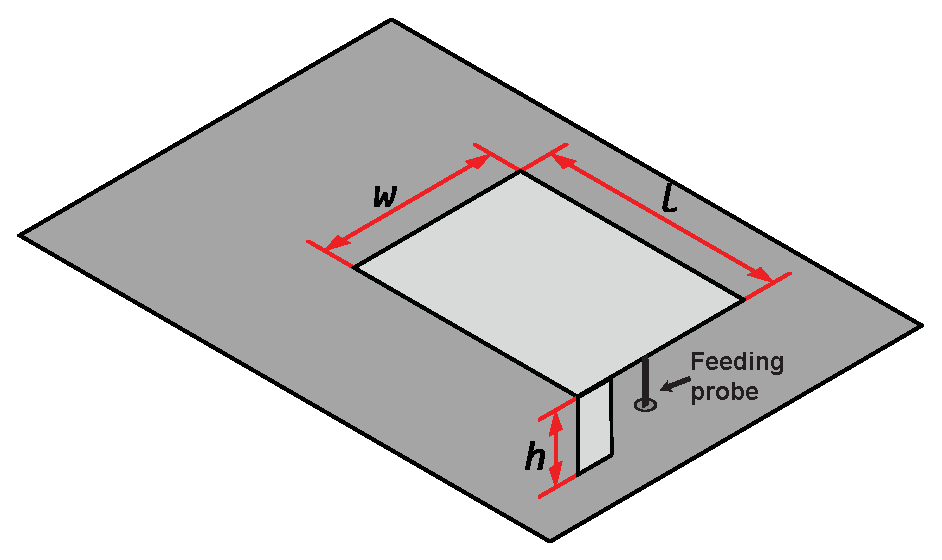
\includegraphics[width=0.5\textwidth]{img/pifa.eps}
    \caption{An illustration of a planar inverted F antenna.}
    \label{fig:pifa}
\end{figure}

\subsubsection{Capacitive coupling elements}
\label{sec:cce}
As all the previously presented antennas are of self-resonant type, capacitive coupling elements (CCE) are categorized as nonresonant antennas. Of course the element resonates at some frequency, but with suitable matching circuits the element is made to resonate at other than its nominal frequency \cite{valkonen_cce}. Capacitive coupling elements were first introduced in \cite{vainikainen_resonator_analysis} as a possible replacement for self-resonant antennas in mobile phones. A great advantage of CCEs is that the size of an antenna can be reduced significantly, considering that self-resonant antennas require rather large amount of space at low frequencies. 

The concept of capacitive coupling elements is explained in \cite{vainikainen_resonator_analysis, villanen_cce}. The basic idea behind them is to combine the wave modes of the antenna and the chassis. This would result enhanced bandwidth for the mobile terminal. For strong coupling to the dominating characteristic wave modes of the chassis, the maxima of electric fields of the antenna and the chassis must be close to each other. Moreover, the volume of the antenna should be used as efficiently as possible to maximize the field strength around the antenna element. PIFAs for example, are not optimal structures for this purpose. 

In contrary to self-resonant antennas, coupling elements are not the main radiators of the system, as presented in \cite{villanen_cce}. The dominant wave mode of the chassis is much stronger than the same wave mode excited by the coupling element, which makes the ground plane the main radiator. With good matching circuitry, it is possible to excite multiple wave modes for broad operational band \cite{valkonen_cce}.


\subsection{Multiantenna systems}
\label{sec:multiant}
Mobile phones today have several radio systems for different applications, and the operating frequencies of them range from hundreds of megahertz to few gigahertz, in the future even to dozens of gigahertz \cite{20ant}. The wide range of required frequencies usually demands for multiple antennas. Generally, these multiantenna systems are multiport systems, which can be distinguished in a few different ways \cite{multiantenna_mimo_book}. The most intuitive one is a multielement antenna, in which each port is connected to physically distinct antenna elements (Figure \ref{fig:mea}). If a single antenna element is fed from several ports, the different antennas can be separated by different polarizations or radiation patterns (Figure \ref{fig:mma}). Additionally, a multiantenna system can also be a combination of these different types.

\begin{figure}[H]
    \vspace{-10pt}
    \centering
    \begin{subfigure}[b]{0.49\textwidth}
        \begin{circuitikz}
            \draw (0,0) node[antenna]{};
            \draw (0,0) node[label={below:Port 1}] {};
            \draw (1.5,0) node[antenna]{};
            \draw (1.5,0) node[label={below:Port 2}] {};
            \draw (4,0) node[antenna]{};
            \draw (4,0) node[label={below:Port $N$}] {};
            \draw (2.75,-0.25) node[label={below:...}] {};
        \end{circuitikz}
        \caption{Multiple separate antennas.}
        \label{fig:mea}
    \end{subfigure}
    \begin{subfigure}[b]{0.49\textwidth}
        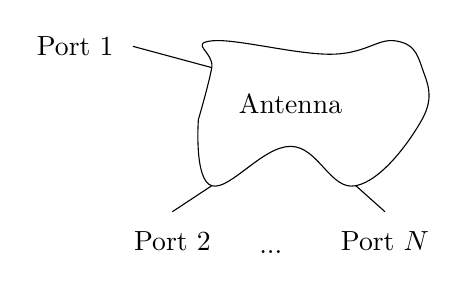
\begin{tikzpicture}
            \draw plot[thick,smooth, tension=.7] coordinates {(-1.17,0.17) (-1,0.83) (-1,1.17) (0.5,1) (1.33,1.17) (1.67,0.83) (1.67,0.17) (0.83,-0.67) (0,-0.17) (-1,-0.67) (-1.17,0.17)};
            \draw (-2,1.1) node[label={left:Port 1}] {};
            \draw (-2,1.1) -- (-1,0.83);
            \draw (-1.5,-1) node[label={below:Port 2}] {};
            \draw (-1.5,-1) -- (-1,-0.67);
            \draw (1.2,-1) node[label={below:Port $N$}] {};
            \draw (1.2,-1) -- (0.83,-0.67);
            \draw (-0.25,-1.25) node[label={below:...}] {};
            \draw (0,0) node[label={Antenna}] {};
        \end{tikzpicture}
        \caption{Single antenna with multiple ports.}
        \label{fig:mma}
    \end{subfigure}
    \caption{Illustrations of multiantenna systems \cite{multiantenna_mimo_book}.}
    \label{fig:multiantennas}
\end{figure}

Multiantenna systems, especially multielement antennas operating at the same frequencies, are also known as multiple input, multiple output (MIMO) communication systems. They can enhance the capacity and bandwidth in wireless transmission \cite{multiantenna_mimo_book}, and exploit the spatial dimension of the channel, which has benefits such as robustness against fading and interference, and improve the signal power \cite{mimo_cellular_networks}. Use of multiple antennas enables transmission of several data streams simultaneously, even at the same frequency by combining diversity or beamforming techniques \cite{volakis}.

In a general communication link, the signal undergoes a multipath process, where the signal is reflected or scattered from various objects on the propagation path. Due to this effect, the electromagnetic waves are received from several directions, and this causes fading that lowers the signal strength \cite{saunders,volakis}. MIMO systems take advantage of this fading, as they collect energy from all the incoming streams, and sum them up. If the antennas are uncorrelated, the fading can be overcome \cite{volakis}.

Antenna diversity can indeed improve the performance of a communications system, if besides good input matching, also the mutual coupling of the antennas is minimized. Isolation of antennas is required for better efficiency, which improves the quality of the link \cite{high_order_mimo}. Envelope correlation coefficient (ECC, $\rho_e$) expresses this information \cite{ecc_paper,mimo_sibille}. ECC is the correlation between the envelopes of the signals for any two antennas of the multiantenna system \cite{mimo_sibille, high_order_mimo}. It is defined by and calculated from the field patterns of the antennas. Calculating ECC from the fields is a demanding task, and in \cite{ecc_paper} an equation to gather the information from the $S$-parameters has been derived
\begin{equation}
\label{eq:ecc}
    \rho_e = \frac{|S_{11}^*S_{12}+S_{21}^*S_{22}|^2}{(1-(|S_{11}|^2+|S_{21}|^2))(1-(|S_{22}|^2+|S_{12}|^2))}.
\end{equation}

This equation is valid for lossless systems, but it can be used as an approximation for lossy structures, similarly to (\ref{eq:eff_aprx}). ECC is used to evaluate the MIMO capability of a multiantenna system, and a coefficient below 0.5 is considered as good performance \cite{reduce_ecc,reduce_ecc2}.


\clearpage